%% using_orthologue_prediction.tex
%% Author: Leighton Pritchard
%% Copyright: James Hutton Institute
%% A brief introduction to orthologues, and evaluation of their prediction

% SUBSECTION: Why orthologues?
\subsection{Using orthologue predictions}

% Which methods work best
\begin{frame}
  \frametitle{Functional adaptation in \textit{Pba}\footnote{\tiny{Toth \textit{et al}. (2006) \textit{Ann. Rev. Phytopath.} \textbf{44}:305-336 \href{http://dx.doi.org/10.1146/annurev.phyto.44.070505.143444}{doi:10.1146/annurev.phyto.44.070505.143444}}}}
  \begin{center}
      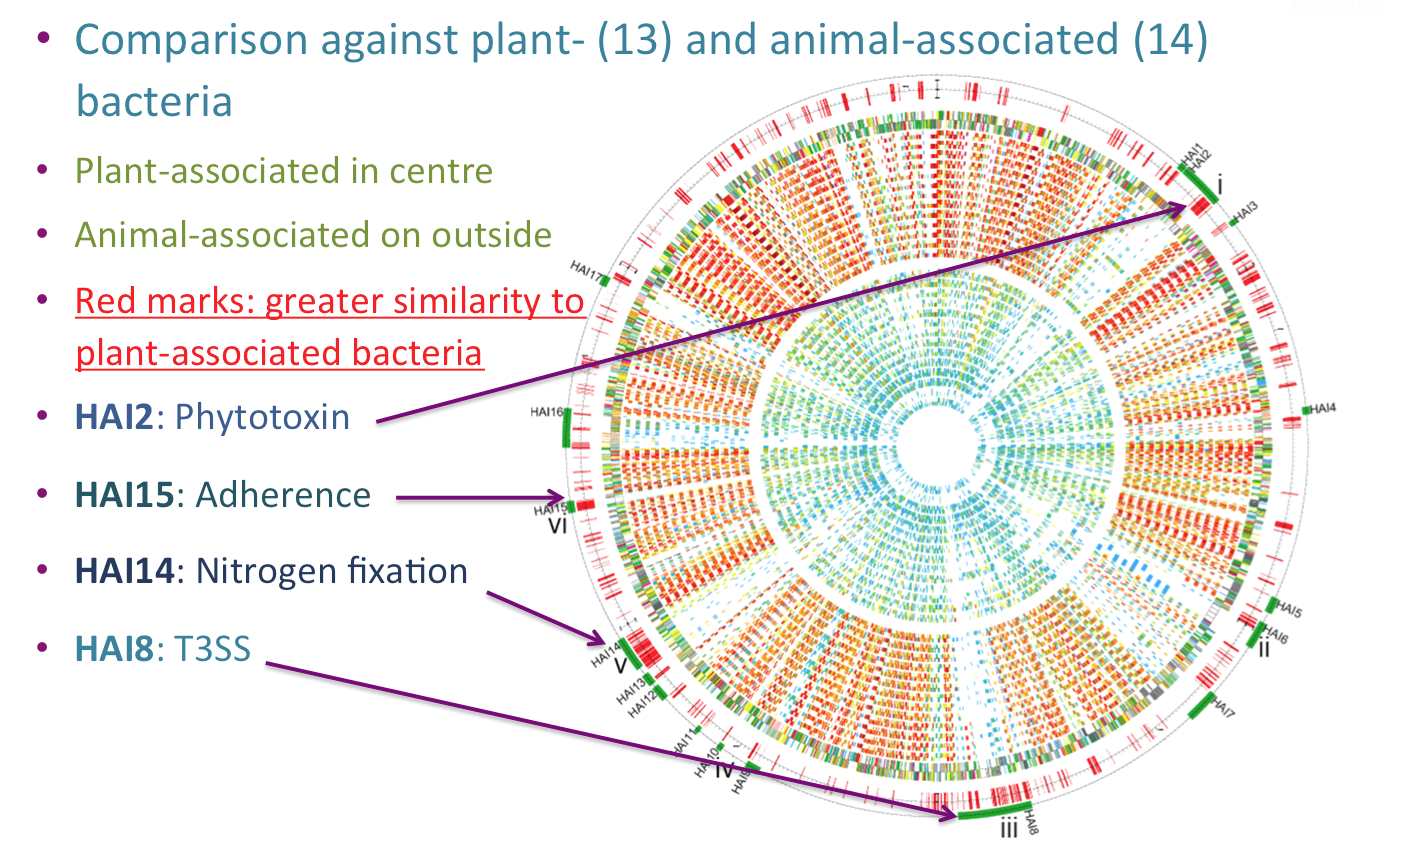
\includegraphics[width=1\textwidth]{images/pba_lgt} 
  \end{center}
\end{frame}

% Which methods work best
\begin{frame}
  \frametitle{Functional adaptation in \textit{Pba}\footnote{\tiny{Toth \textit{et al}. (2006) \textit{Ann. Rev. Phytopath.} \textbf{44}:305-336 \href{http://dx.doi.org/10.1146/annurev.phyto.44.070505.143444}{doi:10.1146/annurev.phyto.44.070505.143444}}}}
  \begin{center}
      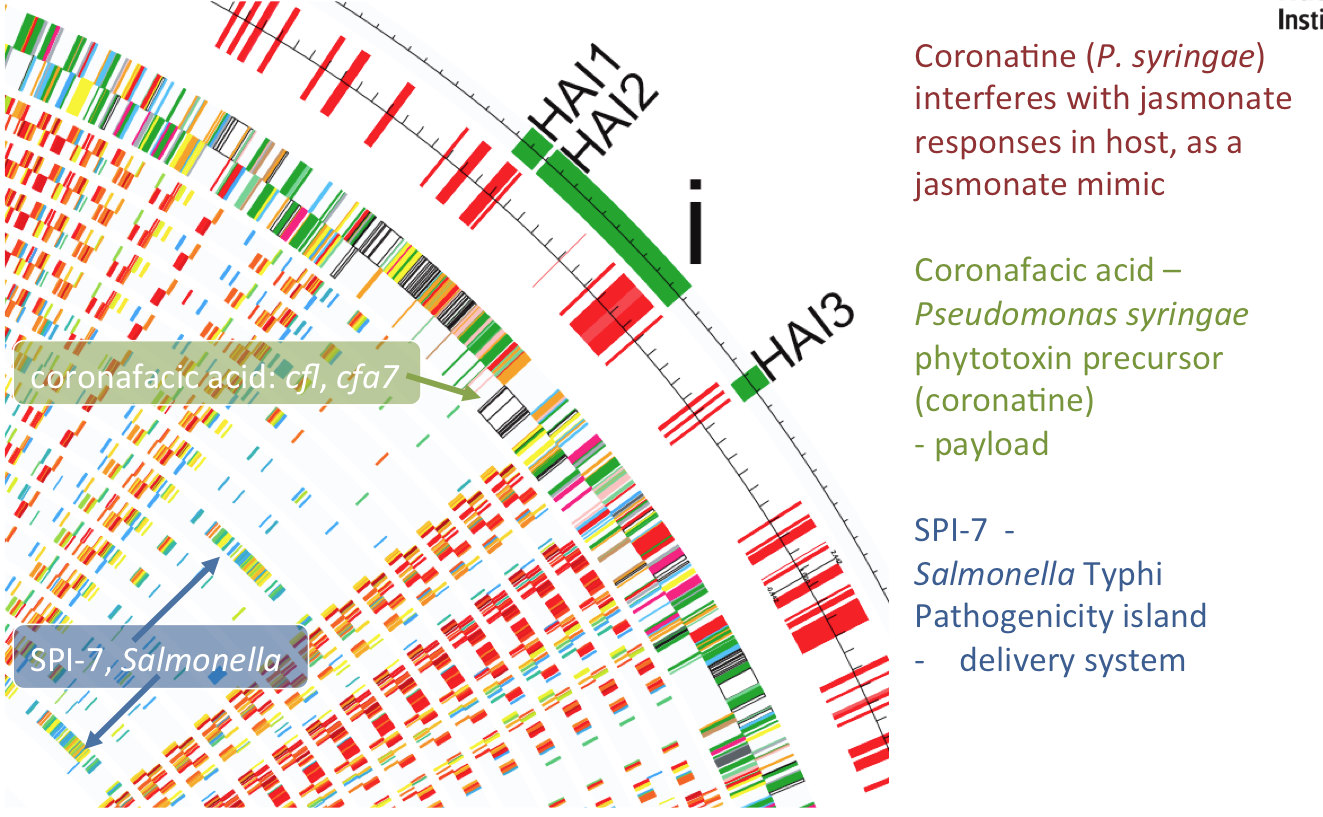
\includegraphics[width=1\textwidth]{images/pba_coronatine} 
  \end{center}
\end{frame}

% SUBSECTION: Core and pangenomes
\subsection{Core and Pan-genomes}

\begin{frame}
  \frametitle{Functional adaptation in \textit{Pba}\footnote{\tiny{Toth \textit{et al}. (2006) \textit{Ann. Rev. Phytopath.} \textbf{44}:305-336 \href{http://dx.doi.org/10.1146/annurev.phyto.44.070505.143444}{doi:10.1146/annurev.phyto.44.070505.143444}}}}
  \begin{center}
      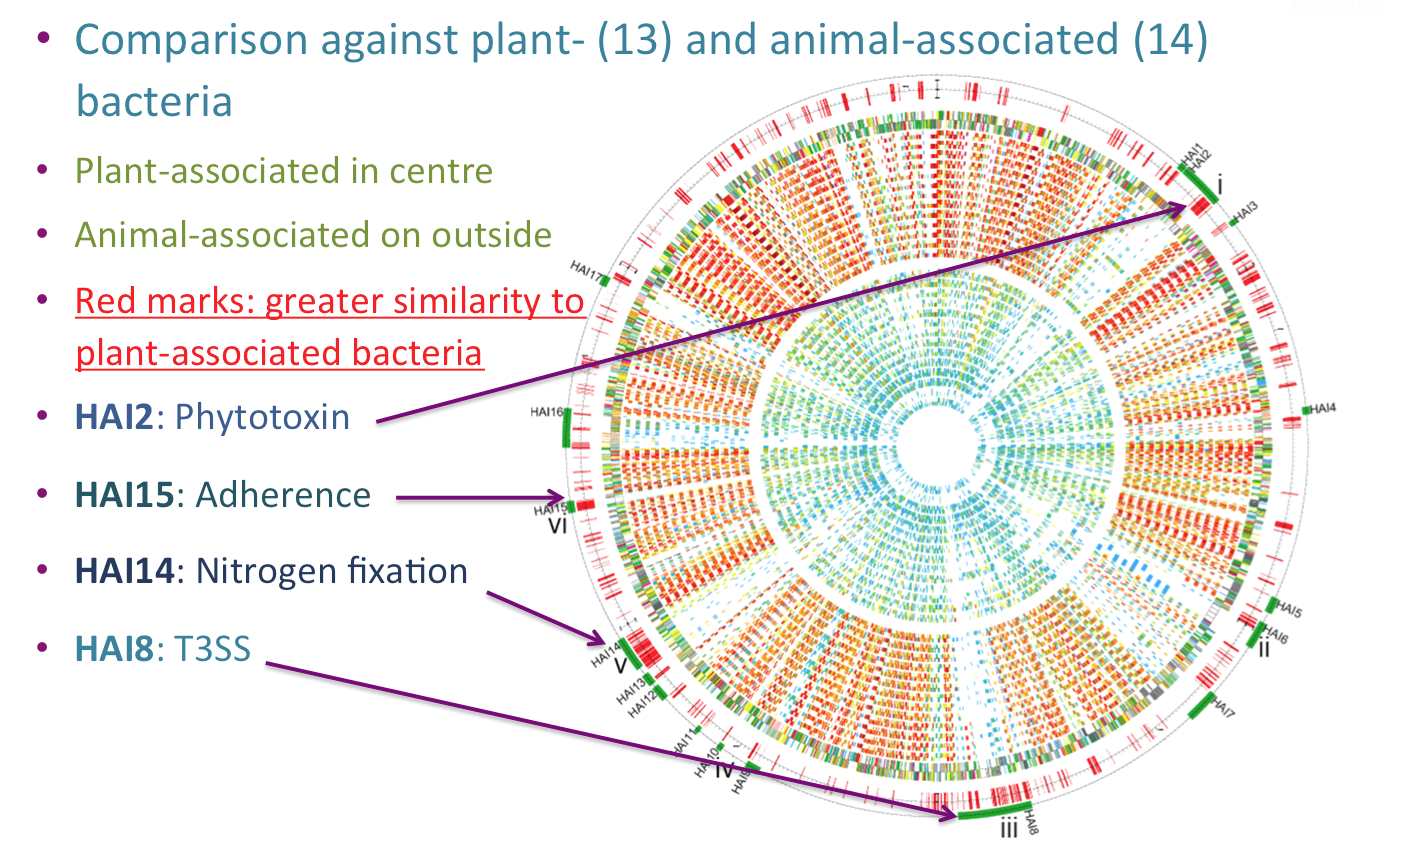
\includegraphics[width=1\textwidth]{images/pba_lgt} 
  \end{center}
\end{frame}

